\begin{figure}
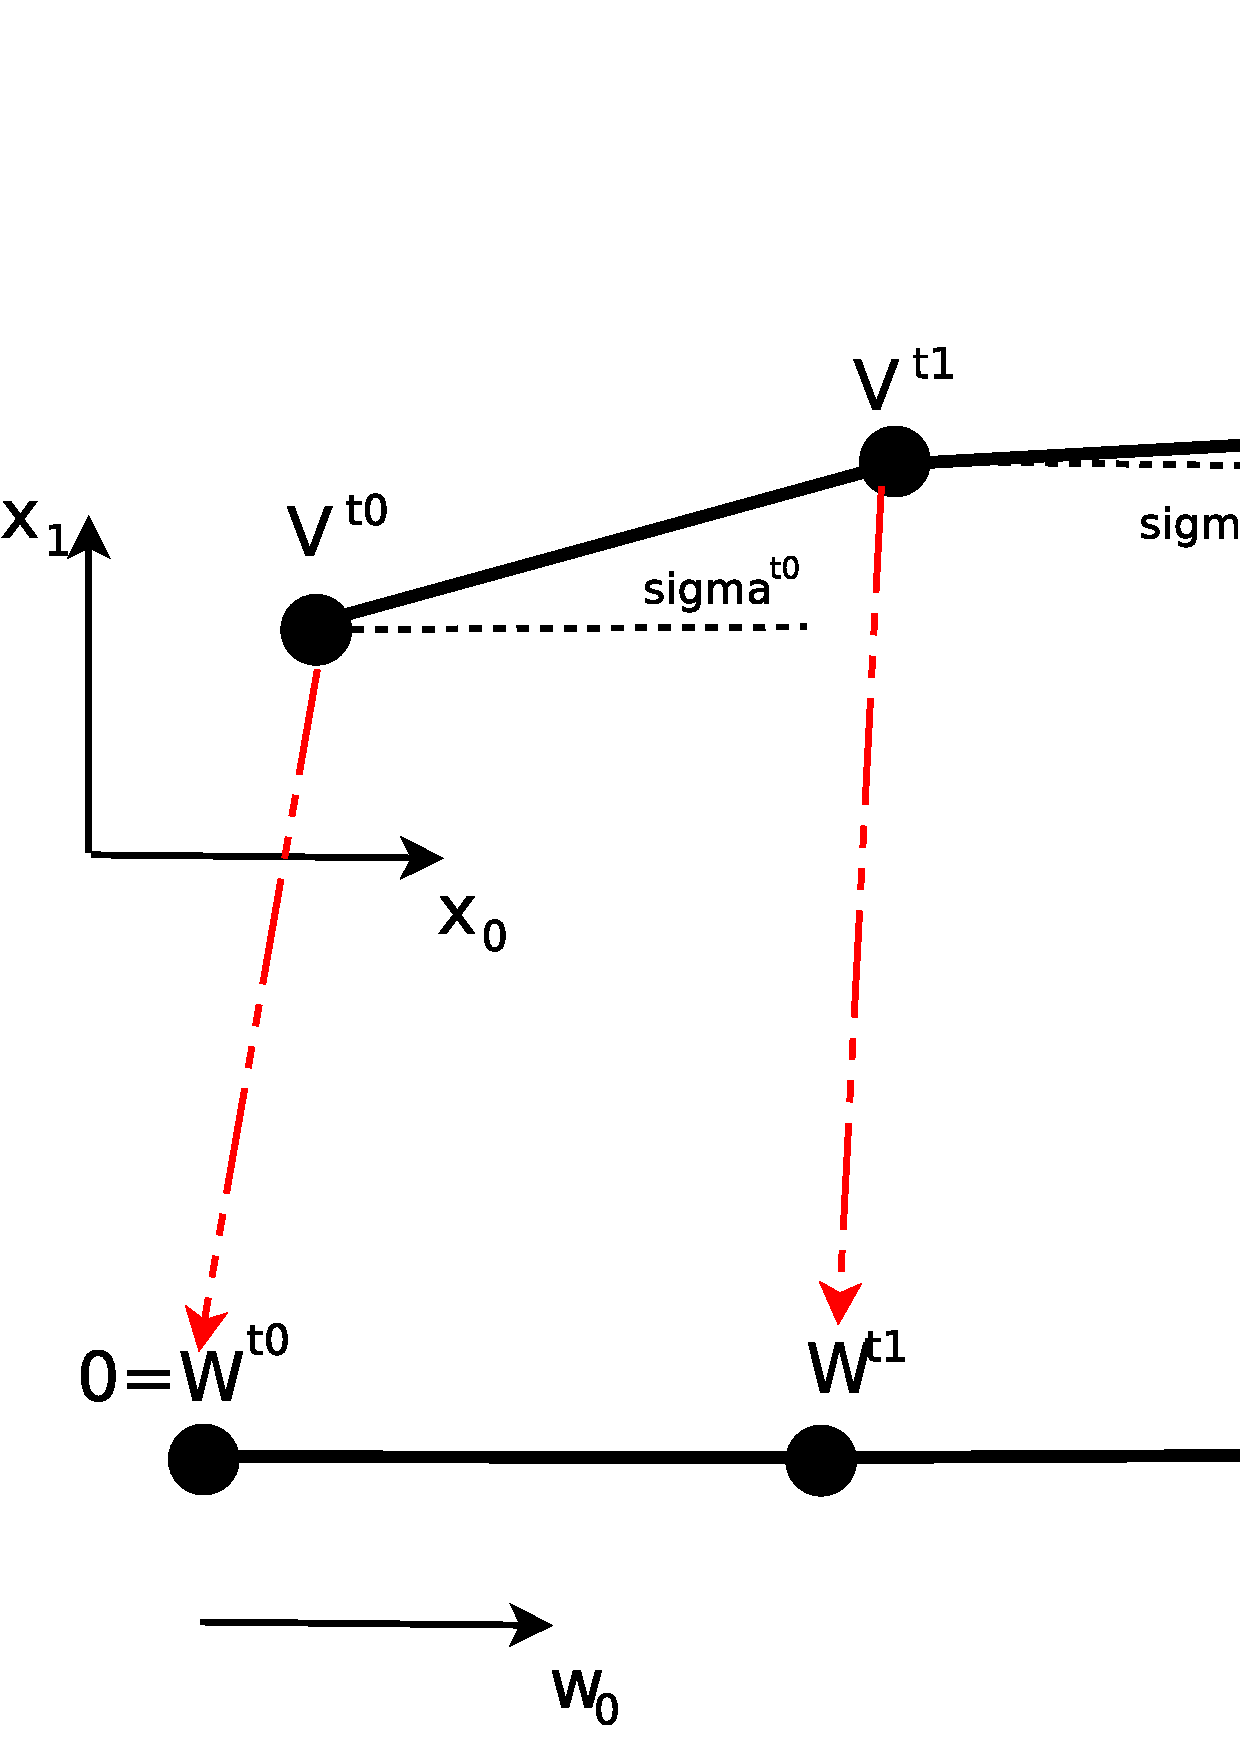
\includegraphics[width=\textwidth]{figures/FaultSystem2D}
\caption{\label{FAULTSYSTEM2D}Two dimensional fault system with one fault named `t` in the $(x\hackscore{0},x\hackscore{1})$ and its parametrization in the
$w\hackscore{0}$ space. The fault has three segments.}
\end{figure}

\section{Fault System}
The \class{FaultSystem} is an easy to use interface to handle 2D and 3D fault systems \index{faults} as used for instance in simulating fault ruptures. The main purpose of the class is to provide a parametrization of an individual fault in the system of fault. In case of a 2D fault the fault is parametrized by a single value $w\hackscore{0}$ and in the case of a 3D fault two parameters $w\hackscore{0}$ and $w\hackscore{1}$ are used. Thsi parametrization can be used
to impose data (e.g. a slip distribution) onto the fault. It can also be a useful tool to visualize or analyse the results on the fault if the fault is not straight. 

A fault $t$ in the fault system is represented by two polygons $(V^{ti})$ and $(v^{ti})$
defining the top and bottom line of the fault $t$.
$V^{ti}$ defines the $i$-th fault vertex at the top of the fault (typically at the surface of the Earth) and
$v^{ti}$ defines the $i$-th fault vertex at the bottom of the fault. Both polygons need to contain the same number of 
vertices. For the 2D case the polygon $(v^{ti})$ for the bottom edge of the fault is dropped. 
The patch with the vertices 
$V^{t(i-1)}$, $V^{ti}$
$v^{t(i-1)}$, and $v^{ti}$
is called the $i$-th segment of the fault `t`. In 2D the the line with the start point $V^{t(i-1)}$ 
and the end point $V^{ti}$ is called the $i$-th segment, see Figure~\ref{FAULTSYSTEM2D}.

In general a fault does not define a plane surface (or a straight line in 2D). In order to simplify working on 
a fault in a fault system a parametrization $P^t: (w\hackscore{0},w\hackscore{1}) \rightarrow (x\hackscore{0},x\hackscore{1},x\hackscore{2})$ over a rectangular domain is introduced such that 
\begin{equation}
0\le w\hackscore{0} \le w^t\hackscore{0 max} \mbox{ and }  -w^t\hackscore{1max}\le w\hackscore{1} \le 0
\label{eq:fault 1}
\end{equation}
with positive if numbers $w^t\hackscore{0 max}$ and $w^t\hackscore{1 max}$. Typically one chooses
$w^t\hackscore{0 max}$ to be the unrolled length of the fault
$w^t\hackscore{1 max}$ to be the mean value of segment depth. Moreover we have 
\begin{equation}
P^t(W^{ti})=V^{ti}\mbox{ and } P^t(w^{ti})=v^{ti}\
\label{eq:fault 2}
\end{equation}
where 
\begin{equation}
W^{ti}=(d^{ti},0) \mbox{ and } w^{ti}=(d^{ti},-w^t\hackscore{1 max})
\label{eq:fault 3}
\end{equation}
and $d^{ti}$ is the unrolled distance of $W^{ti}$ from $W^{t0}$. In the 2D case $w^t\hackscore{1 max}$ is set to zero and therefore the second component is dropped, see Figure~\ref{FAULTSYSTEM2D}.

In the case of 2D the parametrization $P^t$ is constructed as follows:
The line connecting $V^{t(i-1)}$ and $V^{ti}$ is given by
\begin{equation}
x=V^{t(i-1)} + s \cdot (V^{ti}-V^{t(i-1)})
\label{eq:2D line 1}
\end{equation}
where $s$ is between $0$ and $1$. The point $x$ is on $i$-th fault segement if and only if 
such an $s$ esxists. If assume $x$ is on the fault one can calculate $s$ as
\begin{equation}
s = \frac{ (x- V^{t(i-1)})^t \cdot (V^{ti}-V^{t(i-1)}) }{\|V^{ti}-V^{t(i-1)}\|^2} 
\label{eq:2D line 1b}
\end{equation}
We then can set
\begin{equation}
w\hackscore{0}=d^{ti}+s \cdot (d^{ti}-d^{t(i-1)})
\label{eq:2D line 2}
\end{equation}
to get $P^t(w\hackscore{0})=x$.
It remains the question if the given $x$ is actual on the segment $i$ of fault $t$. To test this $s$ is restricted 
between $0$ and $1$ (so if $s<0$ $s$ is set to $0$ and if $s>1$ $s$ is set to $1$) and the we check the 
residual of equation~\ref{eq:2D line 1}, ie. $x$ is been accepted to be in the segement if
\begin{equation}
\|x-V^{t(i-1)} - s \cdot (V^{ti}-V^{t(i-1)}) \| \le tol \cdot max(\|V^{ti}-V^{t(i-1)}\|, \|x-V^{t(i-1)} \|) 
\label{eq:2D line 3}
\end{equation}
where $tol$ is a given tolerance.

ADD DISCRIPTION FOR 3D case.

\subsection{Functions}

\begin{classdesc}{FaultSystem}{
\optional{dim =3}}
Creates a fault system in the \var{dim} dimensional space.
\end{classdesc}



\begin{methoddesc}[FaultSystem]{getDim}{}
returns the spatial dimension
\end{methoddesc}
\begin{methoddesc}[FaultSystem]{getLength}{tag}
returns the unrolled length of fault \var{tag}.
\end{methoddesc}

\begin{methoddesc}[FaultSystem]{getDepth}{tag}
returns the medium depth of fault \var{tag}.
\end{methoddesc}

\begin{methoddesc}[FaultSystem]{getTags}{}
returns a list of the tags used by the fault system
\end{methoddesc}

\begin{methoddesc}[FaultSystem]{getW0Range}{tag}
returns the range of the parameterization in $w\hackscore{0}$.
For tag $t$ this is the pair $(d^{t0},d^{tn})$ where $n$ is the number of segments in the fault.
In most cases one has $(d^{t0},d^{tn})=(0,w^t\hackscore{0 max})$.
\end{methoddesc}

\begin{methoddesc}[FaultSystem]{getW1Range}{tag}
returns the range of the parameterization in  $w\hackscore{1}$.
For tag $t$ this is the pair $(-w^t\hackscore{1max},0)$.
\end{methoddesc}

\begin{methoddesc}[FaultSystem]{getW0Offsets}{tag}
returns the offsets for the parametrization of fault \var{tag}.
For tag \var{tag}=$t$ this is the list $[d^{ti}]$.
\end{methoddesc}


\begin{methoddesc}[FaultSystem]{getFaultSegments}{tag}
returns the polygons used to describe fault \var{tag}. For \var{tag}=$t$ this is the list of the vertices
$[V^{ti}]$ for the 2D and the pair of lists of the top vertices $[V^{ti}]$ and the bottom vertices  $[v^{ti}]$ in 3D.
Note that the coordinates are represented as \numpyNDA objects.
\end{methoddesc}

\begin{methoddesc}[FaultSystem]{getCenterOnSurface}{}
returns the center point of the fault system at the surfaces. In 3D the calculation of the center is
considering the top edge of the faults and projects the edge to the surface (the $x\hackscore{2}$ component is assumed to be 0). An \numpyNDA object is returned.
\end{methoddesc}

\begin{methoddesc}[FaultSystem]{getOrientationOnSurface}{}
returns the orientation of the fault system in RAD on the surface ($x\hackscore{2}=0$ plane) around the fault system center.
\end{methoddesc}
\begin{methoddesc}[FaultSystem]{transform}{\optional{rot=0, \optional{shift=numpy.zeros((3,)}}}
applies a shift \var{shift} and a consecutive rotation in the $x\hackscore{2}=0$ plane.
\var{rot} is a float number and \var{shift} an \numpyNDA object.
\end{methoddesc}

\begin{methoddesc}[FaultSystem]{addFault}{top, tag \optional{, bottom=None \optional{, w0_offsets=None\optional{, w1_max=None}}}}
adds the  fault \var{tag} to the fault system. 

\var{top} is the list of the vertices defing the top of the fault
while \var{bottom} is the list of the vertices defing the bottom of the fault.
In the case of 2D \var{bottom} must not be present. Both list, if present, must have the same length.
\var{w1_max} defines the range of the $w\hackscore{1}$. If not present the mean value over the depth of 
all segement edges in the fault is used.
\var{w0_offsets} sets the offsets $d^{ti}$. If not present it i schoosen such that $d^{ti}-d^{t(i-1)}$ is the length of the $i$-th segment. In some cases, eg. when kinks in the fault are relevant, it can be useful
to explicitly specify the offsets in order to simplify the signamnt of values.
\end{methoddesc}

\begin{methoddesc}[FaultSystem]{getMaxValue}{f\optional{, tol=1.e-8}}
returns the maximum value of \var{f}, the fault wher the maximum is found and the location on the fault in fault coordinates. \var{f} must be a \Scalar. When the maximum is calculated only \DataSamplePoints are considered
which are on a fault in the fault system in the sense of condition~\label{eq:2D line 3} or \label{eq:3D line 3}, respectively. In the case no \DataSamplePoints is found the returned tag is \var{None} and
the maximum value as well as the location of the maximum value are undefined.
\end{methoddesc}

\begin{methoddesc}[FaultSystem]{getParametrization}{x,tag \optional{\optional{, tol=1.e-8}, outsider=None}}
resturns the argument $w$ of the parameterization $P^t$ for \var{tag}=$t$ to provide \var{x}
together with a mask indicating where the given location if on a fault in the fault system by the value $1$ (otherwise the value is set to $0$). \var{x} needs to be \Vector or \numpyNDA object. \var{tol} defines the tolerance to decide if a given \DataSamplePoints is on fault \var{tag}. The value
\var{outside} is the value used as a replacement value for $w$ where the corresponding value in \var{x} is not 
on a fault. If not \var{outside} is not present an appropriate value is used.
\end{methoddesc}

\subsection{Example}
See section~\ref{Slip CHAP}








